\documentclass[11pt,letterpaper]{article}
\usepackage[utf8]{inputenc}

%----- Configuración del estilo del documento------%
\usepackage{epsfig,graphicx}
\usepackage[left=2cm,right=2cm,top=1.8cm,bottom=2.3cm]{geometry}
\usepackage{fancyhdr}
\usepackage{lastpage}

\usepackage{xcolor}
\usepackage{soul}
\newcommand{\mathcolorbox}[2]{\colorbox{#1}{$\displaystyle #2$}}

%------ Paquetes para demostraciónes y árboles de derivación ------%
\usepackage{bussproofs}
\usepackage{scalefnt}

%Color bibi
\definecolor{bibi}{RGB}{0,103,148}
% Otros colores

% ------ Paquetes para arboles --------%
\usepackage{bussproofs}

\usepackage{cite}
\usepackage{multicol}
\setlength{\columnsep}{1.5cm}
\setlength{\columnseprule}{.5pt}

\pagestyle{fancy}
\fancyhf{}
\rfoot{\textit{Página \thepage \hspace{1pt} de \pageref{LastPage}}}

%------ Paquetes matemáticos básicos --------%
\usepackage{amsmath}
\usepackage{amssymb}
\usepackage{amsthm}

%------ Paquetes para codigo --------%
\usepackage{verbatim}

\begin{document}
%------ Encabezado -------- %
\begin{center}
    \begin{minipage}{3cm}
    	\begin{center}
    		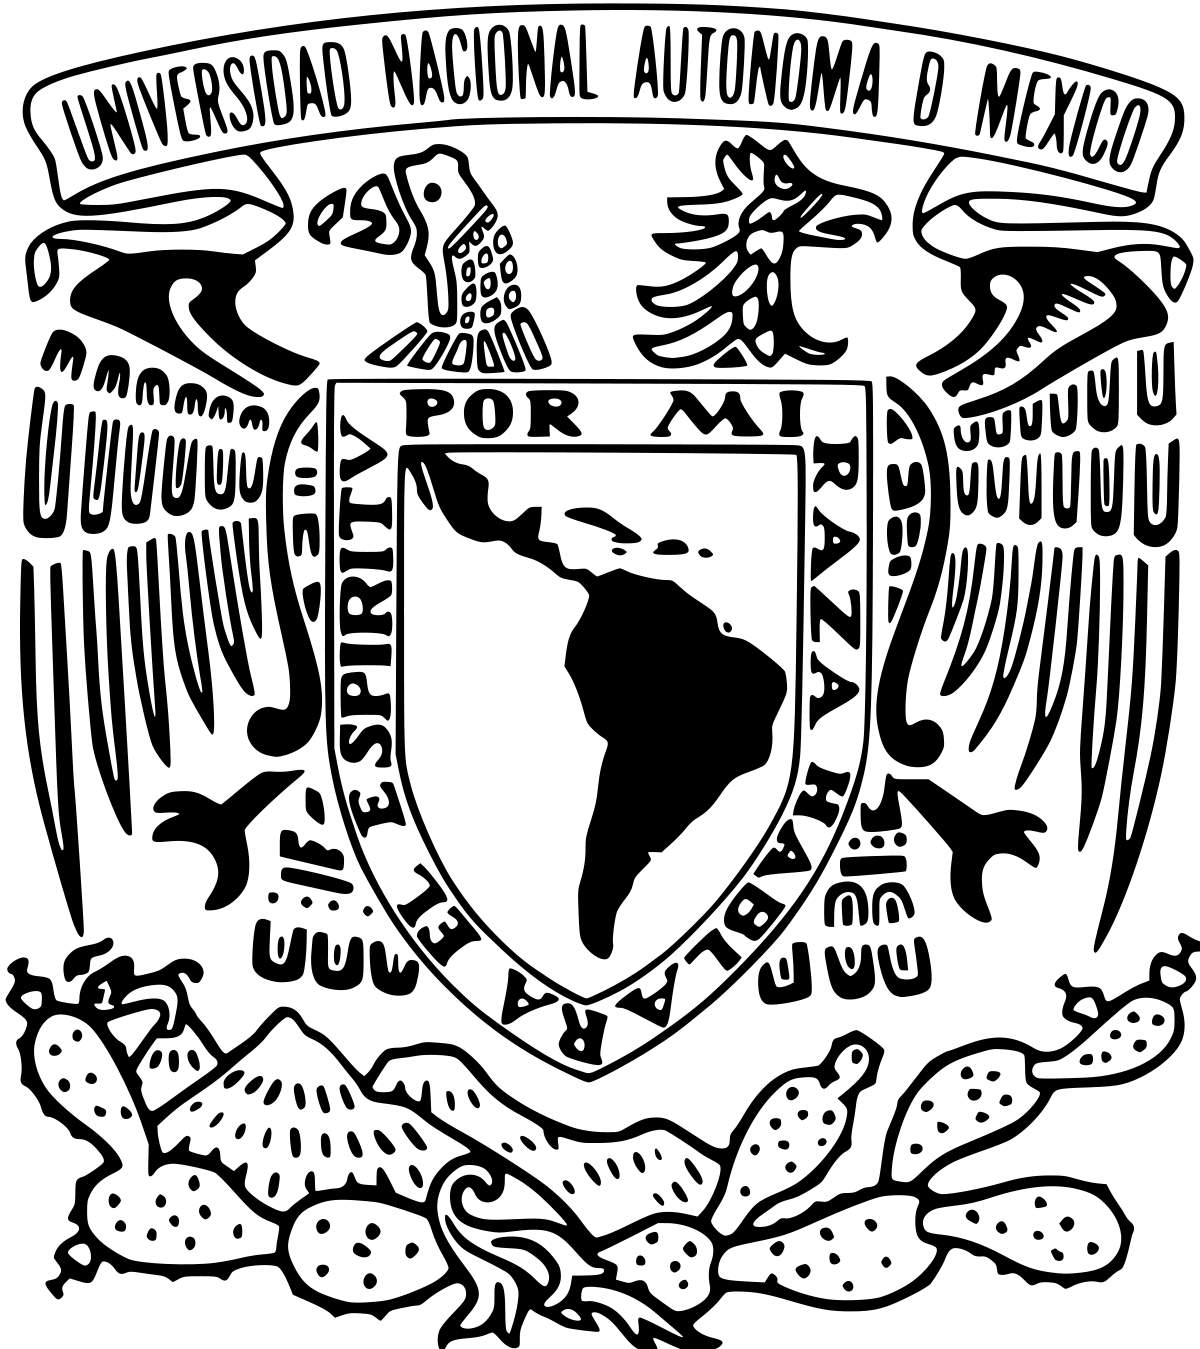
\includegraphics[height=3.4cm]{src/Img/Logo_UNAM.png}
    	\end{center}
    \end{minipage}\hfill
    \begin{minipage}{10cm}
    	\begin{center}
    	\textbf{\large Universidad Nacional Autónoma de México}\\[0.1cm]
        \textbf{Facultad de Ciencias}\\[0.1cm]
        \textbf{Lenguajes de Programación  $|$ 7098}\\[0.1cm]
        Semanal 6 : $|$ Ambientes con diferentes alcances\\[0.1cm]
        Sosa Romo Juan Mario $|$ 320051926 \\[0.1cm]
        Legorreta Esparragoza Juan Luis $|$ 319317532 \\[0.1cm]
        Erik Eduardo Gómez López $|$ 320258211 \\[0.1cm]
        24/09/24
    	\end{center}
    \end{minipage}\hfill
    \begin{minipage}{3cm}
    	\begin{center}
    		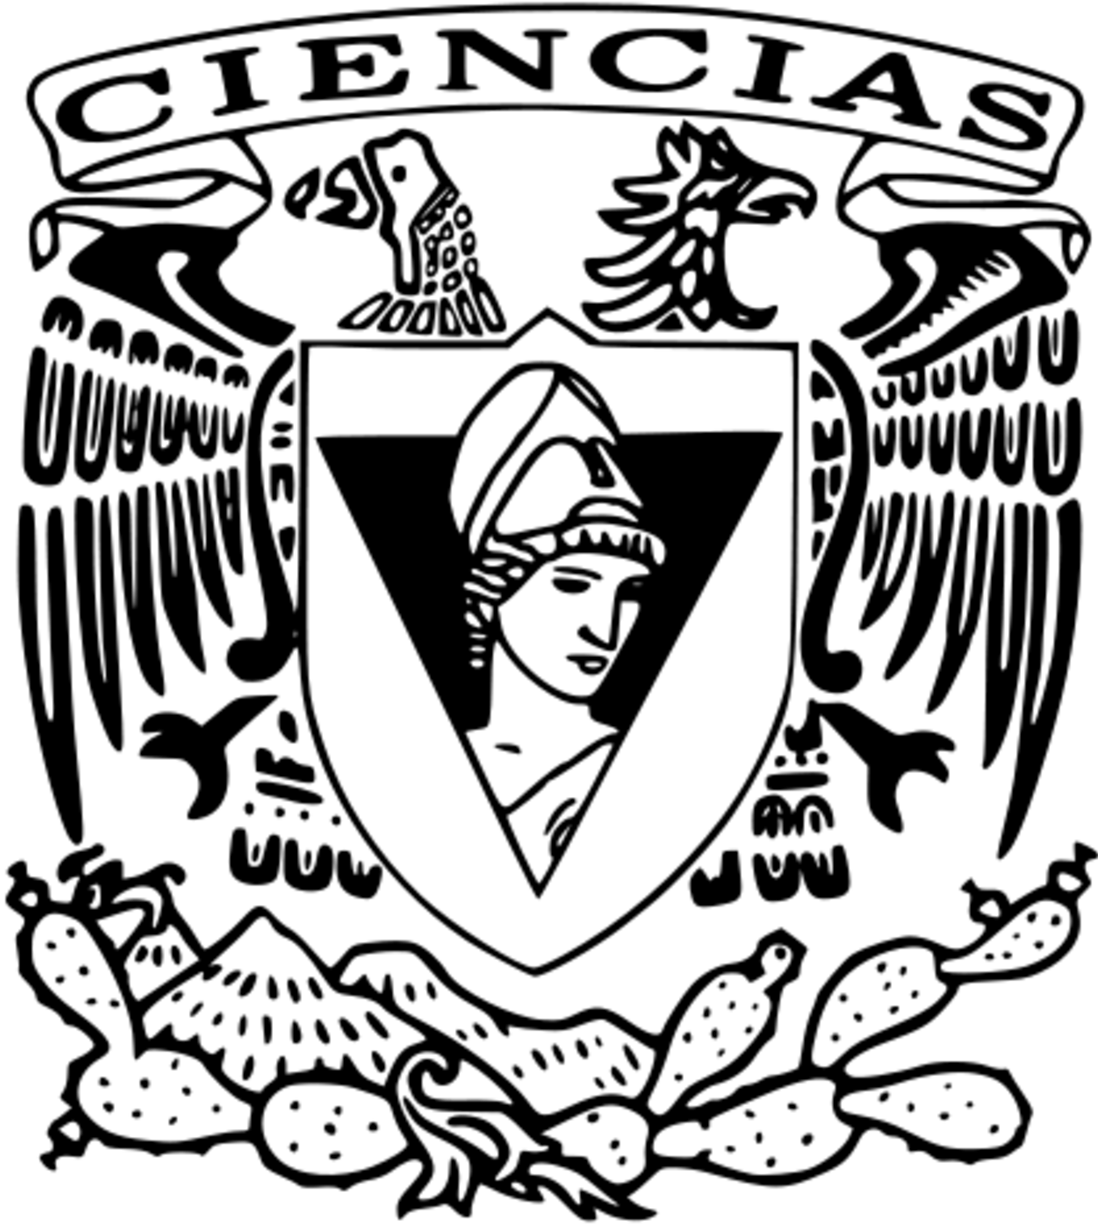
\includegraphics[height=3.4cm]{src/Img/Logo_FC.png}
    	\end{center}
    \end{minipage}
\end{center}


\rule{17cm}{0.1mm}


%------ Ejercicios -------- %
\begin{enumerate}
    \item \begin{verbatim}
    (let (a 2)
        (let (b 3)
            (let (foo (lambda (x) (- (+ a b) x)))
                (let (a -2)
                    (let (b -3)
                        (let (foo (lambda (x) (+ (- a b) x)))
                            (foo - 10)))))))
\end{verbatim}


    \begin{enumerate}
        \item Sustituimos y resolvemos para $a$ y $b$:
\begin{verbatim}
    (let (foo (lambda (x) (- 5 x)))
        (let (a -2)
            (let (b -3)
                (let (foo (lambda (x) (+ (- a b) x)))
                    (foo - 10)))))
\end{verbatim}

Nuevamente sustituimos y resolvemos $(a -2)$ y $(b -3)$ para el siguiente foo:\\
\begin{verbatim}
    (let (foo (lambda (x) (+ (- (-2) (-3) x)))
                    (foo - 10))
\end{verbatim}
Evaluamos:
\begin{verbatim}
    (let (foo (lambda (x) (+ 1 x)))
                    (foo - 10))
\end{verbatim}
El primer $foo$ queda reescrito por el segundo, por lo que lo sustituímos en la expresión final:
\begin{verbatim}
    ((lambda (x) (+ 1 x)) -10)
\end{verbatim}
Evaluamos:
\begin{verbatim}
    (+ 1 -10)
    (-9)
\end{verbatim}
El resultado final es igual a -9.

        \item \textbf{Comenzamos construyendo el ambiente y se queda el cuerpo:}

\vspace{.3cm}

\textbf{Pila:}
\[
\begin{array}{c}
  foo \Leftarrow (lambda (x) (- (+ a b) x))\\
  b \Leftarrow 3 \\
  a \Leftarrow 2 \\
\end{array}
\]

\textbf{Nos queda:}
\begin{verbatim}
(let (a -2)
    (let (b -3)
        (let (foo (lambda (x) (+ (- a b) x)))
            (foo -10))))
\end{verbatim}

Volvemos a agregar los siguientes valores a la pila:

\vspace{.3cm}
\[
\begin{array}{c}
  foo \Leftarrow (lambda (x) (- (+ a b) x))\\
  b \Leftarrow -3 \\
  a \Leftarrow -2 \\
  foo \Leftarrow (lambda (x) (- (+ a b) x))\\
  b \Leftarrow 3 \\
  a \Leftarrow 2 \\
\end{array}
\]

\textbf{Nos queda:}
\begin{verbatim}
    (foo -10)
\end{verbatim}

\textbf{Evaluamos, buscamos el valor de \texttt{foo} en la pila,}

\vspace{.3cm}

\textbf{Nos queda:}
\begin{verbatim}
((lambda (x) (+ (- a b) x)) -10)
\end{verbatim}

Agregamos el valor de $x$ a la pila:
\[
\begin{array}{c}
  x \Leftarrow -10\\
  foo \Leftarrow (lambda (x) (- (+ a b) x))\\
  b \Leftarrow -3 \\
  a \Leftarrow -2 \\
  foo \Leftarrow (lambda (x) (- (+ a b) x))\\
  b \Leftarrow 3 \\
  a \Leftarrow 2 \\
\end{array}
\]

\textbf{Nos queda:}
\begin{verbatim}
(+ (- a b) x)
\end{verbatim}

\textbf{Buscamos los valores de \texttt{a}, \texttt{b} y \texttt{x} en la pila:}

\vspace{.3cm}

\textbf{Nos queda:}
\begin{verbatim}
(+ (- (-2) (-3)) -10)
\end{verbatim}

\textbf{Resolvemos la operación:}

\[
(- (-2) (-3)) = 1
\]

\textbf{Nos queda:}
\begin{verbatim}
(+ 1 -10)
(-9)
\end{verbatim}

El resultado final es -9.

    \end{enumerate}
    \item \begin{verbatim}
    (let (foo (lambda (x) (+ x (foo (- x 1)))))
        (foo 10))
\end{verbatim}

    \begin{enumerate}
        \item Explicar su resultado:
        \item Comenzamos construyendo el ambiente y se queda el cuerpo: \vspace{.3cm}

\textbf{Pila:}
\[
\begin{array}{c}
  foo \Leftarrow (lambda (x) (+ x (foo (- x 1))))
\end{array}
\]

\textbf{Nos queda:}
\begin{verbatim}
    (foo 10)
\end{verbatim}

Evaluamos, buscamos el valor de foo en la pila:

\textbf{Nos queda:}
\begin{verbatim}
    ((lambda (x) (+ x (foo (- x 1)))) 10)
\end{verbatim}

Agregamos a la pila el parametro con su valor y seguimos con el cuerpo:\vspace{.3cm}

\textbf{Pila:} 
\[
\begin{array}{c}
    x \Leftarrow 10 \\
    foo \Leftarrow (lambda (x) (+ x (foo (- x 1))))
\end{array}
\]

\textbf{Nos queda:}
\begin{verbatim}
    (+ x (foo (- x 1)))
\end{verbatim}

Buscamos los valores de x y foo en la pila: \vspace{.3cm}

\textbf{Nos queda:}
\begin{verbatim}
    (+ 10 ((lambda (x) (+ x (foo (- x 1)))) (- x 1)))
\end{verbatim}

Agregamos a la pila el parametro con su valor y seguimos con el cuerpo:\vspace{.3cm}

\textbf{Pila:}
\[
\begin{array}{c}
    x \Leftarrow (- x 1) \\
    x \Leftarrow 10 \\
    foo \Leftarrow (lambda (x) (+ x (foo (- x 1))))
\end{array}
\]

\textbf{Nos queda:}
\begin{verbatim}
    (+ 10 (+ x (foo (- x 1))))
\end{verbatim}

Buscamos los valores de x y foo en la pila: \vspace{.3cm}

\textbf{Nos queda:}
\begin{verbatim}
    (+ 10 (+ (- x 1) ((lambda (x) (+ x (foo (- x 1)))) (- x 1))))
\end{verbatim}

Aqui vemos un problema, la función foo se llama recursivamente, 
ademas el valor de x se esta redefiniendo en la pila,esto combinado
con que no hay caso base, nos lleva a un bucle infinito.
    \end{enumerate}
    \item Realizar los siguientes ejercicios en Haskell:
    \begin{enumerate}
        \item Definir la función recurisva ocurrenciasElementos que toma
como argumentos dos listas y devuelve una lista de parejas, 
en donde cada pareja contiene en su parte izquierda un elemento 
de la segunda lista y en su parte derechael número de veces que 
aparece dicho elemento en la primera lista. Por ejemplo:

\begin{verbatim}
    > ocurrenciasElementos [1,3,6,2,4,7,3,9,7] [5,2,3]
    [(5,0),(2,1),(3,2)]
\end{verbatim}

Yo llegue a la siguiente solución, que usa una función auxiliar
para contar la cantidad de veces que aparece un elemento en una
lista:
\begin{verbatim}
    -- Ocurrencias.hs
    cuentaElemento :: Int -> [Int] -> Int
    cuentaElemento _ [] = 0
    cuentaElemento x [y]
        | x == y    = 1
        | otherwise = 0
    cuentaElemento x (y:ys)
        | x == y    = 1 + cuentaElemento x ys
        | otherwise = cuentaElemento x ys

    ocurrenciasElementos :: [Int] -> [Int] -> [(Int, Int)]
    ocurrenciasElementos _ [] = []
    ocurrenciasElementos xs (y:ys) = (y, cuentaElemento y xs) : 
                                                    ocurrenciasElementos xs ys
\end{verbatim}

La idea es que la función ocurrenciasElementos recorre la lista
de elementos a contar y por cada elemento llama a la función
cuentaElemento que cuenta la cantidad de veces que aparece el
elemento en la lista. La función cuentaElemento recorre la lista
de elementos y por cada elemento compara si es igual al elemento
a contar, si es así suma 1 al contador y sigue con el resto de la
lista, si no es igual sigue con el resto de la lista. Cuando la
lista esta vacía devuelve el contador.

\vspace{.3cm}
        \item Mostrar los registros de activación generados por la 
función definida en el ejercicio anterior con la llamada 
ocurrenciasElementos [1,2,3] [1,2].
        \item Optimizar la función definida usando recursión de cola. 
Deben transformar todas las funciones auxiliares que utilicen.
        \item Mostrar los registros de activación generados por la versión 
de cola con la misma llamada.

\begin{verbatim}
    ocurrenciasElementos2 [1,2,3] [1,2]

    ocurrenciasElementos' [1,2,3] [1,2] []

    ocurrenciasElementos' [1,2,3] [2] ([] ++ [(1, cuentaElemento2 1 [1,2,3])])
    cuentaElemento2 1 [1,2,3] = cuentaElemento' 1 [1,2,3] 0

    ocurrenciasElementos' [1,2,3] [2] ([] ++ [(1, cuentaElemento2 1 [1,2,3])])
    cuentaElemento' 1 [1,2,3] 0 = cuentaElemento' 1 [2,3] 1

    ocurrenciasElementos' [1,2,3] [2] ([] ++ [(1, cuentaElemento2 1 [1,2,3])])
    cuentaElemento' 1 [2,3] 1 = cuentaElemento' 1 [3] 1

    ocurrenciasElementos' [1,2,3] [2] ([] ++ [(1, cuentaElemento2 1 [1,2,3])])
    cuentaElemento' 1 [3] 1 = cuentaElemento' 1 [] 1

    ocurrenciasElementos' [1,2,3] [2] ([] ++ [(1, cuentaElemento2 1 [1,2,3])])
    cuentaElemento' 1 [] 1 = 1

    ocurrenciasElementos' [1,2,3] [2] [(1, 1)] [(1, 1)]
    
    ocurrenciasElementos' [1,2,3] [] ([(1, 1)]++ [(2, cuentaElemento2 2 [1,2,3])]) 
    cuentaElemento2 2 [1,2,3] = cuentaElemento' 2 [1,2,3] 0

    ocurrenciasElementos' [1,2,3] [] ([(1, 1)]++ [(2, cuentaElemento2 2 [1,2,3])])
    cuentaElemento' 2 [1,2,3] 0 = cuentaElemento' 2 [2,3] 0

    ocurrenciasElementos' [1,2,3] [] ([(1, 1)]++ [(2, cuentaElemento2 2 [1,2,3])])
    cuentaElemento' 2 [2,3] 0 = cuentaElemento' 2 [3] 1

    ocurrenciasElementos' [1,2,3] [] ([(1, 1)]++ [(2, cuentaElemento2 2 [1,2,3])])
    cuentaElemento' 2 [3] 1 = cuentaElemento' 2 [] 1

    ocurrenciasElementos' [1,2,3] [] ([(1, 1)]++ [(2, cuentaElemento2 2 [1,2,3])])
    cuentaElemento' 2 [] 1 = 1

    ocurrenciasElementos' [1,2,3] [] ([(1, 1)]++ [(2, 1)])
    [(1, 1), (2, 1)]

\end{verbatim}

Lo escribi maso menos para que se entendiera pero basicamente,
aqui la pila es cuando estan juntas, como vemos en este caso
se va a mantener un solo registro en la pila de llamadas por 
cada función que se llama, y se va a usar una lista o un int
para ir guardando resultados, al final el resultado es el mismo
y la cantidad de operaciones tambien lo es pero se va a mantener
un solo registro en la pila de llamadas.
    \end{enumerate}
\end{enumerate}

\end{document}